\documentclass[11pt]{article}

\usepackage{booktabs}
\usepackage{dcolumn} 
\usepackage{epstopdf}
\usepackage{fourier}
\usepackage{fullpage}
\usepackage{graphicx}
\usepackage{hyperref}
\usepackage{longtable} 
\usepackage{natbib}
\usepackage{rotating}
\usepackage{tabularx}
\usepackage{amsmath}
\usepackage{algorithmic} 
\usepackage{algorithm2e}

\hypersetup{
  colorlinks = TRUE,
  citecolor=blue,
  linkcolor=red,
  urlcolor=black
}

\begin{document} 

\title{Too Clever By (About) $\frac{1}{2}$: \\ 
Excessive Sorting in an Empirical Congestion Game} 

\date{\today}

\author{ John J. Horton \\ NYU Stern \footnote{ Author contact information, datasets and code are currently or will be available at \href{http://www.john-joseph-horton.com/}{http://www.john-joseph-horton.com/}. } }
\maketitle

\begin{abstract}
\noindent  A congestion game was played in which the number of other players was varied, as was the number of ``applications'' per player. 
Players systematically over-compensate for the presence of other players: 
they choose a mixed strategy response that puts too little weight on higher-valued prizes.
Allowing multiple applications does not improve the result.  
\newline 
\newline 
\noindent JEL J01, J24, J3
\end{abstract} 

\section{Introduction}

% Is this just the winner's curse? 

A congestion game is one with defined players and resources and the payoff to an individual depends on how many other players also choose to apply to that resources \citep{monderer1996potential}. 
Many important phenomena can be modeled as a congestion game: applying to colleges, applying for a particular job (or generally deciding who to pursue in a matching market), sending an article to a particular journal and so on. 

% How thick the competition depends upon others assessments of how thick the competition is. 

Even if players play the game rationally, they still generate friction. 
In fact, rational play can lower social efficiency (the Braes paradox). 
In matching models of the labor market, this over and
under-subscription 

\cite{milchtaich1996congestion} 
\cite{chien2011convergence} 

The purpose of this experiment is to understand how individuals play congestion games when the number of other players varies. 
Since in many settings, individuals can have multiple applications, I also have a scenario where they can apply to two prizes. 


Players were told that for each prize, a winner would be selected at random among the ``applicants.''  

\cite{horton2011online} 

\section{Experimental design and game description} 
I ran a \emph{hypothetical} congestion game on MTurk, with five prizes: 
there were four (4) prizes of \$100 each and one prize of \$50. 
Players were told that for each prize, a winner would be selected at random among the ``applicants.''  
They were also told they would be competing against either 0, 1, 10, 25 or 100 other players. 
The experimental interface is shown in Appendix~\ref{TK}, Figure~\ref{TK}. 

Each player should pursue a mixed strategy over the prizes. 
For each prize $i$, a player's probability of application is a function of $x_i$, the prize value. 
In equilibrium, the expectation over each the objects that are applied to with some positive probability should be the same. 
If there are $n$ players, each playing $p(w_i)$ for that object, the count of applications to each object is a binomial random variable, $B(p(w_i), n - 1)$.
For a given set of prizes and number of total players, we can readily compute the mixed strategy for each player by solving 
\begin{equation}
w_i \mathbf{E}\left[\frac{1}{1 + B(p(w_i, n), n - 1)}\right] = k,
\end{equation} 
where $k$ is some constant. 

\section{Results} 

\subsection{One application} 
In Figure~\ref{game_play} I plot the fraction of players choosing one of the \$100 prizes against the NE prediction (dashed line). 
The standard errors for each proportion are calculated using the Wilson method. 
Reassuringly, when the players are playing against no one else, they universally chose \$100. 
They also showed somewhat more subtle reasoning by nearly all picking a \$100 when only one other player played. 
However, we can see that as the number of other players increased, the fraction choosing \$100 fell far below the prediction from the MSNE prediction. 
At $n = 100$, given the empirical distribution of choices, the pay-off to choosing \$100 was more than 30\% higher than the pay-off to choosing \$50. 

\begin{figure}
\caption{Empirical versus theoretical play in the 100-100-100-100-50
  Game, One Application} 
\label{game_play}
\begin{minipage}{0.85\linewidth}
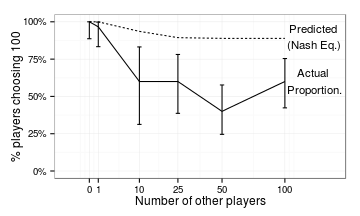
\includegraphics[width = \linewidth]{./plots/comparison100-100-100-100-50.pdf}
\end{minipage} 
\end{figure} 

\subsection{Two applications} 

In Figure~\ref{game_play_2}, I plot the fraction of players choosing to use both of their applications on a \$100 prize. 

\begin{figure}
\caption{Empirical versus theoretical play in the 100-100-100-100-50
  Game, Two Applications} 
\label{game_play_2}
\begin{minipage}{0.85\linewidth}
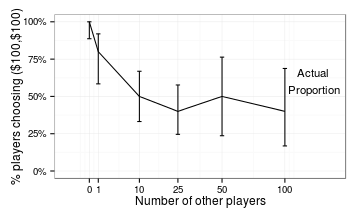
\includegraphics[width = \linewidth]{./plots/comparison100-100-100-100-50_two_apps.pdf}
\end{minipage} 
\end{figure} 

\subsection{Discussion} 

Would feedback help? 

Let's suppose that people play \$100 $p_E$ of the time, and \$50 $1-p_E$ of the time.
Let us also assume that everyone else keeps their play fixed.  

Let us also assume that they start with a prior, $theta$ that $p_E$ is the best strategy to pursue. 

Given the actual empirical play, the best response for the player is actually $(p_{BR}, 1-p_{BR})$. 




After each round, they would only learn whether they one or lost. 

How quickly would they learn? 


When a player plays \$100, their chance of winning is $q_w = \mathbf{E}\left[\frac{1}{B}\right]$. 


Suppose the players starts with beliefs that 

In settings where success is like 
Why? 
Minimize regret? 
Bad at math? 

Repeated play 

Many of the important congestion games 

Learning is likely to be slow. 
If workers thought they had a 50-50 chance of playing the game correctly. 


\section{Conclusion} 


\bibliographystyle{aer}
\bibliography{congestion_game.bib}

\appendix 

\section{Experimental Materials} 

\begin{figure} 
\centering 
\caption{Game interface} 
\begin{minipage}{0.85 \linewidth}
\includegraphics[width = \linewidth]{./images/HIT_interface.png}
\end{minipage} 
\end{figure}  


\end{document} 
